\chapter{Software development is changing}
\label{ch:introduction}
Increased competition and complexity of the problems companies are solving today is changing how software is developed. Software development is getting increasingly more focused towards having short and independent release cycles based on individual features rather than entire applications. Solving complex problems often yield a very complex and fragile solution, but the most successful tech companies have succeeded in utilizing a new architecture pattern that has been named microservices. By creating microservices, changing development process and team structure drastically, modern tech companies create innovative and resilient software quicker than ever seen before.

Several factors has made this new paradigm for developing big scale distributed applications possible. Cloud computing has made it possible to buy computing resources as they are needed, cheap and fast. Virtualization and lately containerization making it possible to create isolated environments, enabling partitioning of applications, into a subset of components that can be developed and deployed independently. The possibility to dynamically orchestrate containers, and ensuring correct capacity and redundancy of application components automatically. Segmentation of the applications in turn makes it possible to maintain a acceptable level of complexity of the source code improving maintainability and increasing agility.

A boom of knowledge sharing throughout the industry, through conference talks and a huge variety of high quality open source projects, together with new programming languages, makes it possible for independent development teams to go from development to deployment very quickly, while taking the complexity of the internet increasingly into account. This has created a new and competitive environment, where understanding and solving complex problems is a process that has to be repeated daily and quickly. Software developers now need to understand the domain and the context they are developing software for in a much higher degree than ever before. 
Having the best and most stable solution to a given problem is not necessarily enough, time to market is extremely important to capture market share as well. New applications need to be available to the customer immediately, and at all times, lack of new features and downtime is immediately visible on the company bottom line.

\section{Microservices}
Monolith applications were a result of technological boundaries, and made developing good design a major challenge. These boundaries have disappeared, pushing developers towards more thoughtful design of applications. Developers today need to put emphasis on understanding the underlying challenges in the particular domain, identifying the optimal architecture that supports the context\cite{evans2016tackling}. High complexity and a strict time to market makes problem solving hard. It is therefore very important to optimize the entire process from identification of a correct solution, through development and deployment of the feature. There are three clear factors in this process: technology utilization, correct working process and organisational structure\cite{george2016it}. Traditionally speaking organisations often divided people into departments according to their specific competences. Each department would be a separated unit, where everyone had the same competences. A new development project would therefore span several departments, creating a need for standardization of tools, languages and working processes. This inherently limits the amount of innovation possible, engineers are forced to solve a problem with a predetermined process, often resulting in similar solutions for very diverse problems\cite{george2016it}. 
Many tech companies have publicly talked about their innovative ways of working, that has allowed them to improve the amount of innovation and the throughput of their software engineers\cite{kniberg2014spotify}. By having a strong focus on having small, strong, cross-functional and self-organising teams that have "end-to-end" responsibility for the features they build. Teams have a overall mission, knowledge of their specific product strategy and short-term goals that help keep the team on the wished path. Each team is given autonomy, responsible for finding the best way for the team to develop new features, which features the team should implement and how they work together. Everyone in the team is located in the same physical location, creating the optimal conditions for good collaboration across skill-sets\cite{kniberg2014spotify}.

\begin{figure}[!htb]
  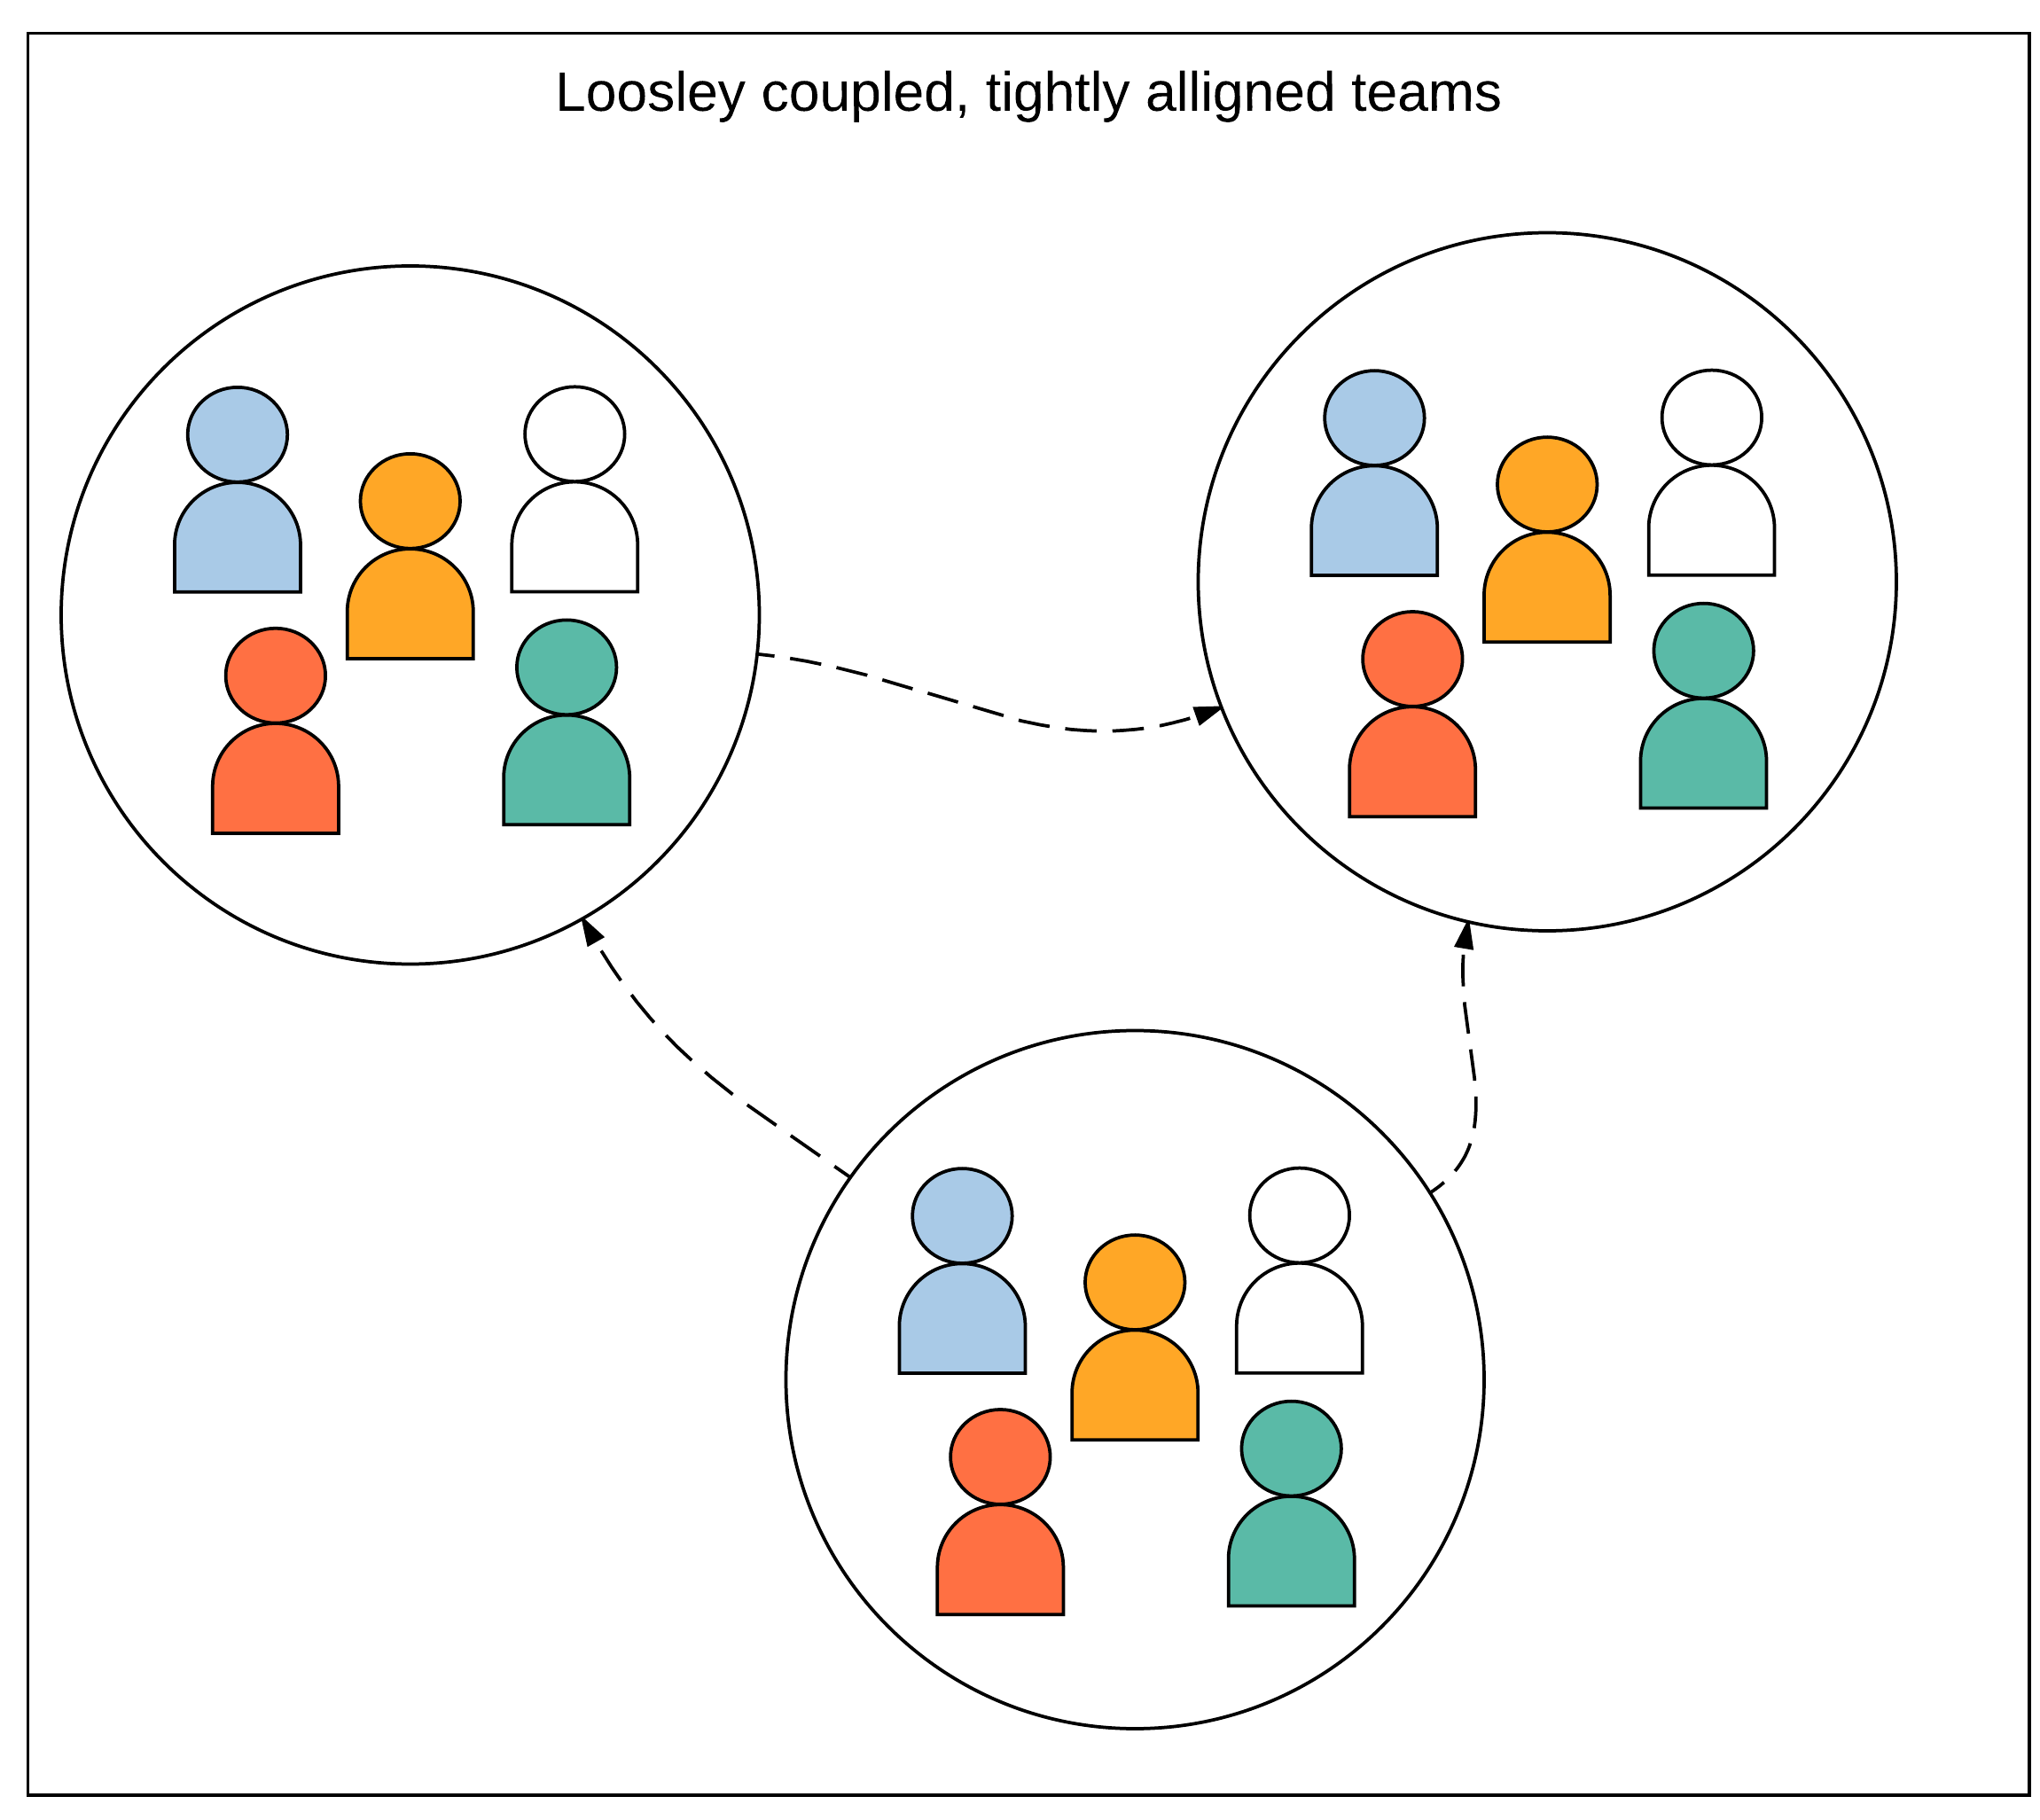
\includegraphics[scale=0.27]{introduction_squads}  
  \caption{Spotify team structure}
  \label{fig:introduction_squads}
\end{figure}

This is a completely new way of designing a organisation, and removes pre-existing process and organisation inhibitors. It is possible for each team to create and release features independently, minimizing waiting time between teams. At the same time teams are responsible for what they create, removing handoffs between teams. The focus is having loosely coupled but tightly aligned teams\cite{kniberg2014spotify}.
It is important that organisation and process inhibitors are removed before utilizing microservices as an architecture choice. This will make it possible to utilize available technology to the fullest, by allowing teams to choose which technology is used for development of the separate features\cite{fowler2014polyglot}. A central database slows down teams, by creating dependencies across team boundaries, creating a need for coordinating changes. Giving the possibility for a polyglot database architecture where a specific database technology is used because of it's advantages in the specific situation creating a system that contains several databases with different data\cite{george2016it, fowler2014microservices}.

\section{Knowledge sharing}
A huge trend of knowledge sharing has started, where online accessible conference talks and a high quantity of open source projects inspire and help developers solve common challenges. Conferences have focus on new open source technology, system architecture, working process and organisational structure, all with a common goal: speeding up software development and the ability to solve increasingly difficult problems. Conferences are either entirely committed to or has tracks about topics like: Cloud computing, Agile development, Domain Driven Design, Microservices, NoSQL, Docker, Cassandra among many others\cite{george2016it}. Company internal projects that beforehand was only internal accessible, are increasingly made open source, giving developers very advanced tools to create elegant and efficient solutions quickly. These projects are freely accessible, with well known support challenges, where developers can find help with specific challenges utilizing the projects.

The entire movement started when Amazon announced Amazon Web Services in 2006. It meant anyone could register and rent virtual machines for hosting distributed applications. Since then, virtualization has been further revolutionised with the introduction of container technology, which was made open source through the docker initiative in 2014. Docker made it possible to start up new independent and isolated environments in seconds, something Google had developed on internally because they needed it\cite{bernstein2014containers}. Which is somewhat a trademark for the entirety of the cloud native movement, is has sprung out of a big variety of needs: serving massive amounts of users, creating reliable applications, the ability to update and add functionality often and easily, minimize integration complexity and technology lock in. In the end the focus should be on solving the problems at hand and in the future, not the maintenance and extension of the existing application.


\section{Resilience}
%Fail whale \url{http://www.whatisfailwhale.info/}
\note {
Distanced view on deployment, focus on development phase
High requirements for availability, always online, always used by users
}





\newpage
\section{Problem formulation}
\label{sc:problem_formulation}

\begin{itemize}  
\item 1.a How can cloud computing be used to solve availability, performance and maintainability requirements for enterprise applications?
\item 1.b How can cloud computing be used in an enterprise application architecture?

\item 2.a How are enterprise application challenges and possible solutions affected by the application domain?
\item 2.b How does the enterprise application domain affect challenges and possible solutions?
\item 2.c How does the domain shape the challenges in a specific application architecture?
\item 2.d How does the domain and organization shape the challenges in a specific application architecture?

\item 3.a How does a distributed application architecture deal with a single point of failure?
\item 3.b How is single point of failure avoided in a distributed application architecture?

\item 3.c How is the optimal application architecture and distribution method determined and evaluated?
\item 3.d How is the enterprise application architecture determined?
\item 3.e How is the enterprise application architecture evaluated?
\end{itemize}

\subsection*{Notes}
How are the challenges and their optimal solution affected by the specific application?

What determines the optimal application architecture, database and distribution?

How is the optimal application architecture, database and distribution determined?

System architecture:
How is application data optimally stored?
How is application data optimally distributed?

How are application updates optimally executed?
How are updates 

How is the system distributed

This area has been named cloud computing, 

Big cloud computing platforms are now available, offering server rental with 

From these requirements big cloud platforms have been started, 

These requirements has started big scale initiatives in cloud computing, has generated new tools and databases available for development of distributed big scale enterprise applications. 

Creating a need for developers to explore and evaluate which of the many platforms to choose, 